\chapter*{Proposition 37}



\begin{figure*}[ht]
    \begin{center}
    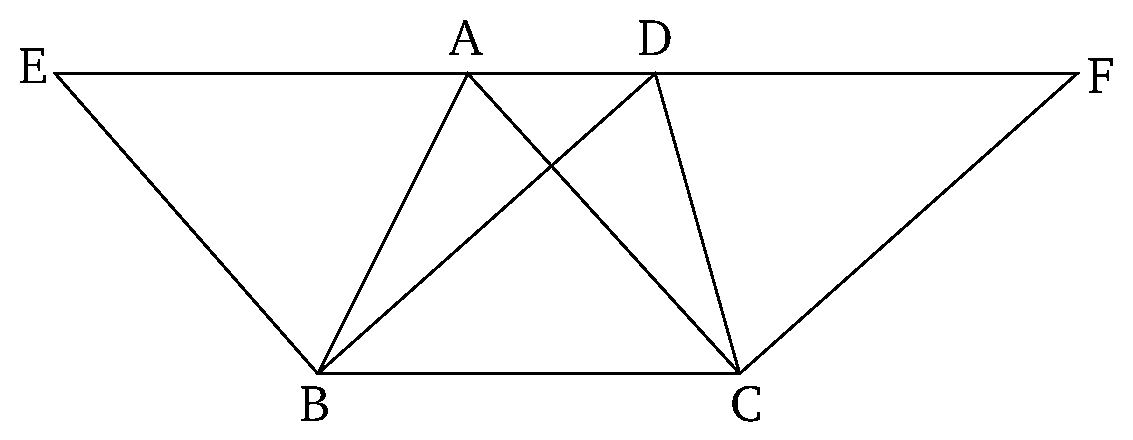
\includegraphics[width=0.5\linewidth]{figures/fig37e.eps}
    \label{fig:prop_37}
    \end{center}
\end{figure*}

Triangles which are on the same base and between the same parallels
are equal to one another.

Let $ABC$ and $DBC$ be triangles on the same base $BC$, and between
the same parallels $AD$ and $BC$. I say that triangle $ABC$ is equal to triangle $DBC$.

Let $AD$ have been produced in both directions to $E$ and $F$, and let the
(straight-line) $BE$ have been drawn through $B$ parallel to $CA$ [Prop.~1.31],
and let the (straight-line) $CF$ have been drawn through $C$ parallel to
$BD$ [Prop.~1.31]. Thus, $EBCA$ and $DBCF$ are both parallelograms,
and are equal. For they are on the same base $BC$, and between
the same parallels $BC$ and $EF$ [Prop.~1.35]. And the triangle $ABC$ is
half of 
the parallelogram
$EBCA$. For the diagonal $AB$ cuts the latter in half [Prop.~1.34]. And the 
triangle $DBC$ (is) half of the parallelogram $DBCF$. For the diagonal
$DC$ cuts the latter in half [Prop.~1.34]. [And the halves of equal things are
equal to one another.]$^\dag$
Thus, triangle $ABC$ is equal to triangle $DBC$.

Thus, triangles which are on the same base and between the same parallels
are equal to one another. (Which is) the very thing it was required to show.


\section*{Commentary}

\begin{proposition}\label{proposition_37}\lean{Elements.Book1.proposition_37}\leanok
    If
\end{proposition}
\begin{proof}
    \uses{proposition_31,proposition_33,proposition_35}\leanok
\end{proof}
